\begin{minipage}[b]{0.45\linewidth}
    \centering
    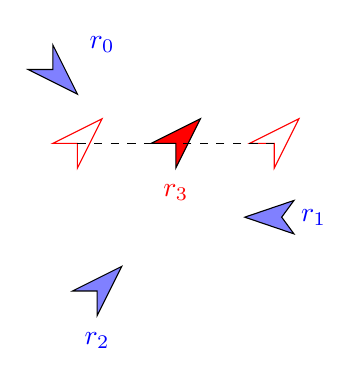
\begin{tikzpicture}[scale=1.25]
      \draw[fill=blue!50] (3.2,2.5) -- (2.95,2.5) -- (3.45,2.75) -- (3.2,2.25)   -- cycle;
      \node[color=blue] at (3.2, 2) {$r_2$};
      % draw grids
      % \draw[color=gray, help lines, line width=.05pt] (-1,1)  grid[xstep=.5cm, ystep=.5cm] (6,6);
      \draw[fill=blue!50] (3,4.5) -- (2.75,5) -- (2.75,4.75) -- (2.5,4.75)   -- cycle;
      \node[color=blue] at (3.25, 5) {$r_0$};
      \draw[fill=blue!50] (5.2,3.42) -- (4.7,3.25) -- (5.2,3.08) -- (5.075,3.25)  -- cycle;
      \node[color=blue] at (5.4,3.25) {$r_1$};    
      \draw[fill=red] (4,4) -- (3.75,4) -- (4.25,4.25) -- (4,3.75) -- cycle;
      \node[color=red] at (4, 3.5) {$r_3$};
      \draw[color=red] (3,4) -- (2.75,4) -- (3.25,4.25) -- (3,3.75) -- cycle;
      \draw[dashed] (3,4) -- (4,4);
      % \draw (0,-4.75) node[below] {reflect across $x$-axis};  
      \draw[color=red] (5,4) -- (4.75,4) -- (5.25,4.25) -- (5,3.75) -- cycle;
      \draw[dashed] (5,4) -- (4,4);
    \end{tikzpicture}
  \end{minipage}
  \begin{minipage}[b]{0.45\linewidth}
    \centering
    \begin{tikzpicture}[scale=1.25]
      \node[] (A) at (4,4)    {$\langle3\rangle$};
      \node[] (B) at (3,2.5)  {$\langle2\rangle$};
      \node[] (C) at (5.5,4)  {$\langle3,1\rangle$};
      \node[] (D) at (3,5)    {$\langle3,0\rangle$};
      \draw[edge] (A) -- (D);
      \draw[edge] (A) -- (C);
    \end{tikzpicture}
  \end{minipage}
  \caption{[left] A root robot $r_3$ has three neighbors, and two outgoing
  edges from its role vertex.  [right] After exchanging messages. Robot $r_3$ selects $r_0$ and $r_1$ as its children since they are two robots who are closest to two desired opening position corresponding to the out-edges. Robot $r_2$ is an orphan without any assignment.}